\section{Materials and Methods}

%{{{ comments 
%The materials and method section should describe in detail the procedures followed, indicating an awareness of any likely pitfalls or problems with the techniques. Published techniques need not be described in detail but should be referenced. The student should demonstrate an understanding of established techniques. \underline{N.B.} no results obtained by the student should appear in this section.
% 
% \begin{itemize}
 % \item Does this section describe in detail the procedures followed? Could you carry out this project following the methods reported here?
% \end{itemize}

% \begin{figure}[h]
	% \begin{center}
    % \includegraphics{es3d.pdf}
	% \end{center}
    % \caption{Example of an embedded pdf}
% \end{figure}
%}}}

%{{{ data sources 
\subsection{Data sources}
% WHERE THE DATA COME FROM
% WHAT THOSE DATA ARE
% FIGURE OF DATA SOURCES -> MYSQL DB WITH NAME OF SCRIPTS
% FIGURE OF DATABASE SCHEMA

The DomVizApp database was built by importing and linking the following sources: Pfam \cite{pfamdb}, Uniprot \cite{uniprot}, PDB \cite{pdb} and Drugbank \cite{drugbank}.

A collection of Perl modules were written to perform data pre-processing and to import the data into a MySQL\footnote{http://www.mysql.com/} database which acts as the master data store. These Perl scripts allow databases to be created given new data from Pfam, Uniprot or the PDB. Importing the data into a general purpose database allows us to easily integrate our data sources, facilitates flexible querying for analysis and allows for additional annotation in the future. The data sources, import scripts and database schema are illustrated in Figure~\ref{dataimport} and described below.  

\begin{figure}[h]
 \begin{center}
 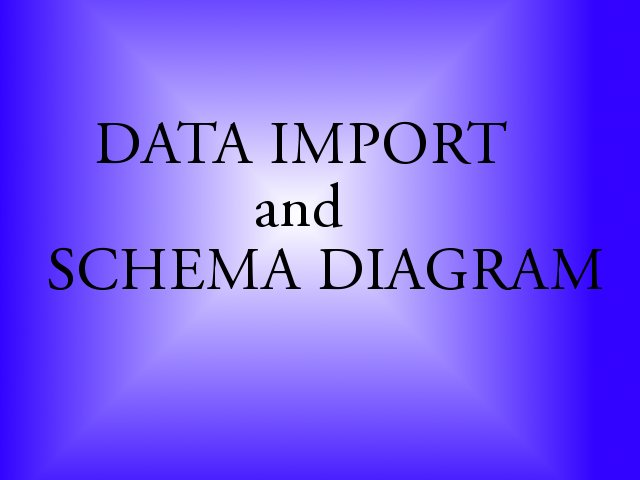
\includegraphics[scale=0.5]{figures/placeholder.jpg}
 \end{center}
 \caption{Overview of data sources and target schema}
 \label{dataimport}
\end{figure}

\subsubsection{Pfam}
Domains and architectures form the foundation of DomVizApp and were imported from Pfam version 22.0, available from the Pfam FTP site\footnote{ftp://ftp.sanger.ac.uk/pub/databases/Pfam/current\_release/swisspfam.gz}. The swisspfam dataset contains all the domains belonging to a sequence. Domains aren't presented linearly and the file requires additional parsing in order to extract the sequence's architecture. We extracted and loaded the sequence accession, Swissprot name and stored the sequence's architecture as a string with a dot-separated format (e.g. \texttt{D1.D2.D3.D1.D1}). The list of all Pfam clans (Pfam-C.gz) was also imported so that those domains that belonged to clans could be associated with other sibling domains. 

The dataset contains 45,684 distinct architectures (ignoring Pfam-B domains) from 9,318 domains, *fillme* of which are members of one of *fillme* clans.

\subsubsection{Uniprot}
In order to link domain architectures to sequences and taxonomy, Uniprot v14.0 (Swissprot 56.0) protein data were imported. The data includes all accession numbers for Swissprot entries, which allows us to link drug targets with Pfam sequence entries. We are also able to group sequences by identical domain organizations. This release contains 392,667 UniprotKB/Swissprot entries. % todo: only swissprot entries?

\subsubsection{PDB}
The PDB records were used to determine protein sequences that have had their structure solved. DomVizApp uses this information to allow users to filter for architectures that belong to a sequence that has had its structure determined. Links between PDB chain and Uniprot are only available in separate downloads for each individual chain from the Worldwide Protein Data Bank (wwPDB). Rather than downloading and parsing the full PDB database, we used the PDBSprotEC mappings \cite{pdbsprotec} which are available from the Bioinformatics Group at UCL\footnote{http://www.bioinf.org.uk/pdbsws/}. The dataset has 110,858 PDB chains mapped to *fillme* distinct Swissprot sequences. 

\subsubsection{DrugBank}
To analyse the targetting of proteins by drugs, details of drugs and their corresponding targets were obtained from the DrugBank \cite{drugbank} drugset as of 14 June 2008. The full drugcard set contains comprehensive drug data combined with drug-target data, such as sequence, Swissprot identifier and GO classification information. It also includes Pfam domains for each of the targets but it simply lists all the domains belonging to the target, not specifically the domains targetted by the drug. Only approved drug targets were considered in the analysis. The full drugcard set lists 4,764 drugs of which 1,484 are flagged as `Approved'. For our analysis, we only considered human targets. 

%}}}

%{{{ data analysis
\subsection{Domain architecture analysis}
% DESCRIBE ANALYSIS PERFORMED
% HOW THEY WERE PERFORMED
% WHY THEY WERE PERFORMED
After loading and integrating the different data sources, and having performed the necessary normalization of Pfam and Drugbank sequence accession numbers to the Uniprot primary accession number, we were able to perform some general analysis of the protein domain and architecture landscape. Using progressively selective criteria, we were able to retrieve summary information related to protein sequence Pfam entries, human protein domains and commonly occuring architectures.

For the first stage of analysis, a collection of SQL scripts were written to summarize the number of distinct domains and architectures and how frequently these domains and architectures occurred in sequences. We extracted this information for all species and HomoSapiens.

We also analysed the occurrences of domains in architectures, which required development of MySQL stored procedures as the information could not be retrieved using standard SQL set operations. We obtained these totals by getting a list of distinct domains and then iteratively searching for architectures that contained these domains. We retrieved total and HomoSapien numbers.

As mentioned previously, the purpose of this analysis was to survey the domain architecture landscape. As DomVizApp draws network graphs of related architectures, we wanted to have a sense of how large a typical graph would be (i.e. number of nodes) and what might be the worst case scenario. We were also able to see what types of domains were frequently occuring and investigate what was their related function.

The second stage of analysis was to investigate the possible number of `druggable' proteins in the human genome. Using the current DrugBank drug-target data we found the number of approved drugs currently targetting human proteins. We then retrieved additional protein sequences that had the same architecture as drug-targets but weren't currently targetted by any drugs.

To improve the number of probable druggable proteins, we should also include those sequences which have some of the domains (or all domains but in a different architecture) that specifically bind the drug. However, Drugbank does not currently state explicitly which domain the drug targets. We calculated the number of sequences that contain one or more of the same domains as the drug-target protein. This is likely to return an inflated figure of druggable targets as it is unlikely that a drug targets all the domains in a target protein.

This shortcoming is a reason that one of the goals of DomVizApp is to assist bioinformaticians to interactively explore protein architectures by allowing them to indicate domains of interest (say, a domain known to bind a drug) and then update the network graph accordingly.

%}}}

%{{{ implementation
\subsection{DomVizApp implementation}
% EVERYTHING THAT THE APPLICATION DOES AND USES
DomVizApp was wriiten in Java, using JDK 1.6. We used the Lucene search toolkit\footnote{http://lucene.apache.org/}, which was used to create high-performance search indexes of the biological data. The Prefuse toolkit \cite{prefuse}, a visualization framework for Java, was used to model graph data and visualize the network graph.

\subsubsection{Data preparation and indexing}
% Details of what the Lucene engine does for you and how exactly you used it for indexing your data
Our master data was stored in MySQL. As the schema was designed for data integrity and to reduce redundancy, its relational nature did not suit general-purpose querying. The performance of SQL queries was not fast enough to give DomVizApp users a highly interactive and dynamic experience. A common solution is to denormalise the data into new tables within MySQL that have been especially created for the types of queries that will be run against it.

As DomVizApp runs as a desktop application, we desired a solution that did not necessarily require the use of MySQL, which would require a database server to be installed and made accessible for the user. A better answer was to generate local, file-based, indexes that could be distributed to users of the application.

Lucene is a library for high-performance creation and searching of text indexes. By taking data from the master MySQL database and producing a Lucene index, we were able to have a separate, transferable, set of files that could be distributed to user's workstations. All the necessary information would be available locally to the user and this would facilitate the dynamic nature of DomVizApp.

The first stage was the indexing of our master data to create a searchable index. A Lucene index is stored as set of index files containing an inverted index data structure that allows rapid searching of text words. We interated through each sequence in Pfam, collecting data associated with it, such as its architecture and whether its structure has been solved, to create a Lucene \texttt{Document} which is a collection of fields. Each piece of Pfam data was stored as a field in the sequence Document.

We similarly created Documents for domain data, holding the Pfam domain identifier and its clan associations. 

Each of these documents was added to the Lucene index. The full workflow is shown in Figure~\ref{luceneworkflow}

\begin{figure}[h]
 \begin{center}
 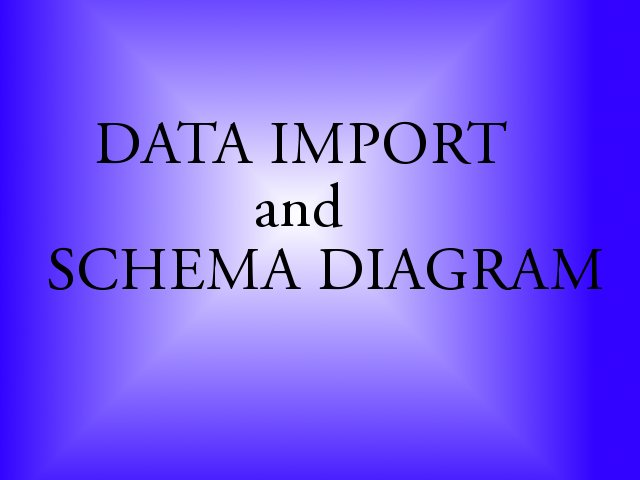
\includegraphics[scale=0.5]{figures/placeholder.jpg}
 \end{center}
 \caption{Lucene indexing workflow}
 \label{luceneworkflow}
\end{figure}

The Lucene index was searched from within DomVizApp based on user's specified criteria. Queries are written in a custom query language which is parsed by the Lucene index searcher. Lucene returns \texttt{Hits} matching the query and a reference to the original Document (e.g. Pfam sequence entry). We extracted the stored fields from these documents and were then able to use the data in DomVizApp.   

The total size of Lucene index was **fillme**Mb. Average query time to return data associated with a Pfam sequence was **fillme**ms and to return architectures containing a random domain took **fillme**ms on average. 

\subsubsection{Network graph visualisation}
% details of what the prefuse engine does for you and how exactly you used it for rendering network graphs. what is involved in customizing it for your application. a figure helps. show different components, highlight those that you need to customize/hack. describe layout techniques and force-directed layout in particular. what is the network graph meant to show
We are using network graphs to visually represent our data and their relationships. Graph visualisation is a fundamental component of DomVizApp and we used the Prefuse framework to both model graph data structures and to display the graph.

The framework provides interfaces and libraries for graph modelling, rendering and layout. Prefuse offers an API to control and customize almost all components of graph visualisation. The are several core components of the Prefuse framework, which are shown in Figure~\ref{prefuseframework} and described below.

\begin{figure}[h]
 \begin{center}
 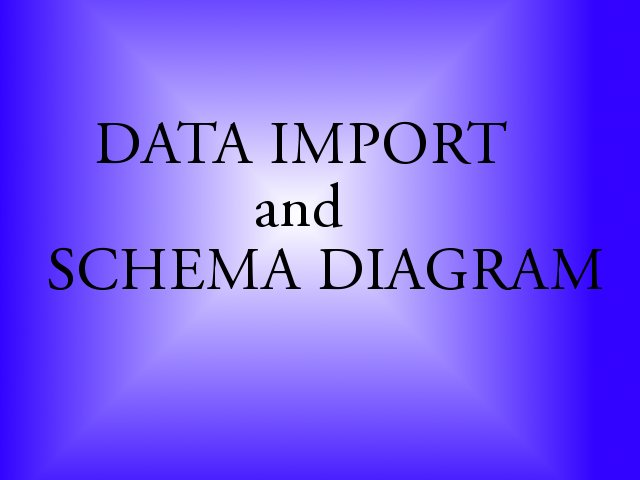
\includegraphics[scale=0.5]{figures/placeholder.jpg}
 \end{center}
 \caption{Components of the Prefuse Framework}
 \label{prefuseframework}
\end{figure}

\textbf{Data representation:} To model architectures and sequences we used the \texttt{Node} class. Their corresponding relationships were modelled using the \texttt{Edge} class. Both Node and Edge classes are subtypes of \texttt{Entity} which can hold any number of named elements with corresponding value. We stored Pfam domain identifiers, architectures, similarity scores and sequence names with their corresponding node or edge. This simplified querying of the graph itself as all biological data related to nodes or edges were stored with the entities themselves. No further lookup for data was required.

\textbf{Visual representation:} We then represented each node and edge as a \texttt{VisualItem}. A VisualItem stores the data related to entities and adds further properties related to the size, colour and other visual attributes. We used a different representation for architecture and sequences so they could be distinguished from each other.

\textbf{Interactions:} Prefuse \texttt{ActionLists} were used to respond to user actions and system events. These included executing the layout algorithm and adding callbacks to users clicking on nodes or edges. We were able to display the attributes of entities and collapse and expand sequence nodes in response.

\textbf{Rendering:} There are several algorithms provided for constructing network drawings and Prefuse allows most aspects of the layout algorithms to be customised. Due to the large number of nodes and edges, typical of bioinformatics datasets, standard graph rendering is tricky and usually not satisfactorily clear. We required not only a clear representation of the graph itself but also needed to be able to visualise features common to a group of architectures. DomVizApp uses a force-directed layout \cite{force}, provided by Prefuse, which attempts to place all the nodes by modelling entities as elements with physical forces that interact with each other. For example, edges have a spring force. All of these forces (gravity, spring and drag) can be customised as required. By simulating these forces across the nodes and edges, the layout brings connected nodes together and spreads unconnected nodes apart until the forces reach equilibrium, resulting in clear and expressive graphs. 

In DomVizApp, this means that two architectures that are similar will be placed closer in the resulting graph than architectures that are less similar. Groups of similar architectures will gather closer together. We customised the spring force of the edges which join architecture nodes and manipulated its properties based on the similarity score of the architectures. This modification brought architectures that are more similar than others closer together in the layout.

As this layout algorithm can be CPU-intensive, we allow the user to stop the the algorithm when a reasonable layout has been acheived. The final graph may not be mathematically the best graph but achieves an elegant layout \cite{force}.

\subsubsection{User interface}
% how it is laid out and what it requires to get started. what is the network graph meant to show
DomVizApp was designed to let bioinformaticians explore sequence architectures easily and clearly. The user interface was designed to encourage exploration through simplicity and responsiveness.

The interface is implemented using Java Swing libraries and the main screen is divided into 3-panes. The left pane is for user input: search, filtering and rendering options. The central pane displays the network graph. The bottom pane displays information about the current view or current user selection.

Users can interact with the graph pane using the mouse. The graph can be dragged, zoomed in or out and elements (nodes and edges) can be selected. Further information related to selected elements is displayed in the bottom pane.

To begin using DomVizApp, a user enters a protein sequence identifier. The application retrieves the architecture of the sequence (the `parent architecture'). It then searches for all architectures that share one or more domains with the parent architecture. These architectures, and sequences with these architectures, are visualised as a network graph. We allow the user to apply further filtering to this graph of results. For example, they may limit results to certain species or specific domains of interest. Because we are searching data held in an index stored locally, DomVizApp is able to quickly respond to changes in user's criteria and render new graphs.

The main component of the user interface is the network graph pane. Visualization of the similarity between architectures allows users to quickly and effectively interpret this information. Architectures and sequences are represented as nodes on the graph. All sequences are connected to their architecture by an edge. Architecture similarities are represented by an edge that connects architecture nodes to other architectures based on the strength of the similarity. We wrote rendering components for Prefuse to animate the addition and removal of nodes to highlight changes in the graph due to changes in criteria. 

%}}}

%{{{ computing architecture similarity
\subsection{Computing the scores for architecture similarity}

Given a set of architectures, all of which share a particular Pfam domain, one can obtain a matrix of all pairwise similarity scores between the architectures. We used such a matrix as the basis of the network graph to arrange architectures according to their relative similarities. We also used the similarity score to manipulate the spring forces for edges in the network graph to create clusters of similar architectures.

For DomVizApp, we used the Needleman-Wunsch algorithm \cite{nwalgo} to calculate this similarity score. The procedure is illustrated in Figure~\ref{computingscores} and described below. 

\begin{figure}[h]
 \begin{center}
 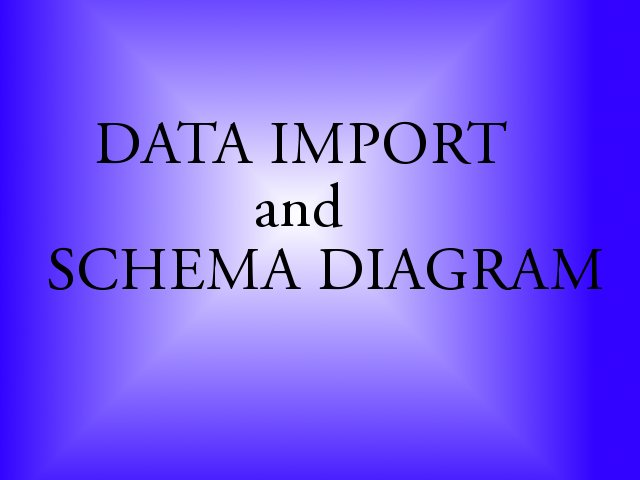
\includegraphics[scale=0.5]{figures/placeholder.jpg}
 \end{center}
 \caption{Calculating the all-against-all pairwise matrix of similarity scores}
 \label{computingscores}
\end{figure}

The first step in comparing any two architectures that share one or more domains was to create a similarity matrix scoring each of the domains present in the architectures. The score assigned to each pair in a similarity matrix may be simple, indicating a straighforward match or mismatch, or it may be related to a more sophisticated heuristic. For example, domain similarities could be measured using one of the techniques mentioned in the Introduction. The different heuristics and scoring techniques would ultimately result in different relationships among sets of architectures and therefore different graphs.

For the current version of DomVizApp, we used a scoring matrix that measures domain similarity based on:
\begin{enumerate}
	\item Domains matching exactly
	\item Domains belonging to the same clan, as defined by Pfam
	\item Domain mismatch
\end{enumerate}

Given the domain similarity matrix, we then used Needleman-Wunsch to perform an alignment of the two architectures based on their sequence of domains and obtain a maximal alignment score.

By applyting this technique for all pairs in a given set of architectures, an all-against-all pairwise matrix of similarity scores is calculated. 
%}}}

%{{{ using matrix of scores to draw network graph
\subsection{Using the matrix of scores to draw the graph}

To create the network graph, the calculated architecture similarity matrix was used to connect each architecture in the set with its highest scoring match. An edge was used to connect the two architecture nodes. 

To begin the process of connecting the architectures, we started with a graph of unconnected nodes. Each of the nodes represented an architecture in our set. First, we connected the parent architecture to its highest scoring match in the matrix. We then iterated over each of the unconnected architectures looking for the highest scoring match among the connected architectures. Once found, this unconnected architecture was joined to the connected architecture. We continued  iterating over unconnected architectures until all architectures had been connected to at least one other node.

If in the process of connecting architectures we found that there was an unconnected architecture which had the same high similarity score for two of more architectures, the architecture was connected to all of the high scoring architectures.
%}}}


